\documentclass[crop,tikz]{standalone}
\usetikzlibrary{backgrounds}
\colorlet{blue}{cyan}
\tikzset{
  inverted/.style = {
    color=white,
    background rectangle/.style={fill},
    show background rectangle
  }
}

\tikzset{>=latex}
\usetikzlibrary{calc}

\begin{document}
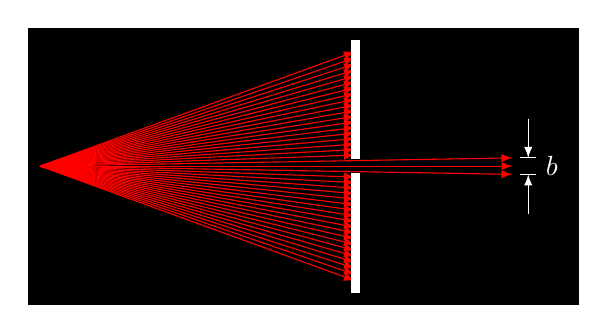
\begin{tikzpicture}[inverted,inverted]
  % rays
  \foreach \d in { -20,-19,...,-2 } { \draw[->,red] (0,0) -- +(\d:{4/cos(\d)}); };
  \foreach \d in {  20, 19,..., 2 } { \draw[->,red] (0,0) -- +(\d:{4/cos(\d)}); };
  \foreach \d in { -1, 0, 1       } { \draw[->,red] (0,0) -- +(\d:6); };
  % aperture
  \draw[fill] (4-0.05,-1.6) rectangle (4+0.05,-0.1);
  \draw[fill] (4-0.05, 0.1) rectangle (4+0.05, 1.6);
  % description
  \draw[]   ($( 1:6)+(0.1,0)$) -- +(0.2,0);
  \draw[]   ($(-1:6)+(0.1,0)$) -- +(0.2,0);
  \draw[->] ($( 1:6)+(0.2, 0.5)$) -- +(0,-0.5);
  \draw[->] ($(-1:6)+(0.2,-0.5)$) -- +(0, 0.5);
  \node[right] at (0:6.3) {$b$};
\end{tikzpicture}
\end{document}
